\newpage


\section{Parallelism and Dependence Theory}

  


\subsection{DATA DEPENDENCE}

\begin{figure}[H]
	\centering
	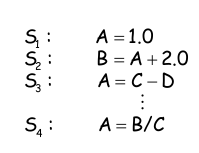
\includegraphics[width=0.3\textwidth]{p197.png}
	\caption{An example.}
	\label{fig:p197}
\end{figure}



    \begin{itemize}
    \item Flow (true) dependence: a statement $S_i$ precedes a
    statement $S_j$ in execution and $S_i$ computes a data value that
    $S_j$ uses. $S_i \delta^{+} S_j$. In Figure \ref{fig:p197}, $S_1 \delta^{+} S_2$ and $S_2 \delta^{+} S_4$

    \item Anti dependence: a statement $S_i$ precedes a statement $S_j$ in
    execution and $S_i$ uses a data value that $S_j$ computes. $S_i \delta^{a} S_j$
    In Figure \ref{fig:p197}, $S_2 \delta^{a} S_3$

    \item Output dependence: a statement $S_i$ precedes a statement $S_j$
    in execution and $S_i$ computes a data value that $S_j$ also
    computes. $S_i \delta^{o} S_j$,
    In Figure \ref{fig:p197}, $S_1 \delta^{o} S_3$ and $S_3 \delta^{o} S_4$
    \end{itemize}


The dependence is said to flow from $S_i$ to $S_j$ because $S_i$
precedes $S_j$ in execution.
$S_i$ is said to be the source of the dependence. $S_j$ is said to
be the sink of the dependence.
The only “true” dependence is flow dependence; it
represents the flow of data in the program.
The other types of dependence are caused by programming
style; they may be eliminated by re-naming as seen in Figure \ref{fig:p198}.


\begin{figure}[H]
	\centering
	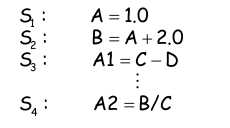
\includegraphics[width=0.3\textwidth]{p198.png}
	\caption{Dependence other than flow dependence can be eliminated by re-naming for Figure \ref{fig:p197}.}
	\label{fig:p198}
\end{figure}



\subsection{DATA DEPENDENCE DIRECTIONS}

\subsubsection{ = }

\begin{figure}[H]
	\centering
	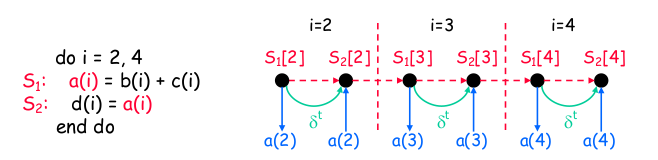
\includegraphics[width=0.3\textwidth]{p199.png}
	\caption{}
	\label{fig:p199}
\end{figure}


In Figure \ref{fig:p199}, There is an instance of $S_1$ that precedes an instance of $S_2$ in
execution and $S_1$ produces data that $S_2$ consumes.
$S_1$ is the {\color{red}source} of the dependence; $S_2$ is the {\color{red}sink} of the
dependence.
The dependence flows between instances of statements in the
same iteration ({\color{red}loop-independent} dependence).
The number of iterations between source and sink (dependence
distance) is 0. The {\color{red}dependence direction} is {\color{red}=}.
$S_1 \delta^{+}_{=} S_2$ or $S_1 \delta^{+}_{0} S_2$

\subsubsection{$<$}

\begin{figure}[H]
	\centering
	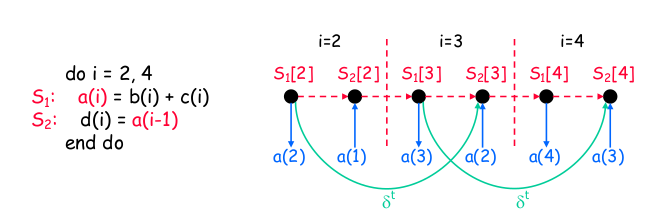
\includegraphics[width=0.3\textwidth]{p200.png}
	\caption{}
	\label{fig:p200}
\end{figure}

In Figure \ref{fig:p200},there is an instance of $S_1$ that precedes an instance of $S_2$ in
execution and $S_1$ produces data that $S_2$ consumes.
$S_1$ is the source of the dependence; $S_2$ is the sink of the
dependence.
The dependence flows between instances of statements in
different iterations (loop-carried dependence).
The dependence distance is 1. The direction is positive (<).
$S_1 \delta^{+}_{<} S_2$ or $S_1 \delta^{+}_{1} S_2$


\subsubsection{$>$}

\begin{figure}[H]
	\centering
	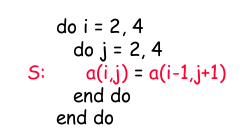
\includegraphics[width=0.3\textwidth]{p201.png}
	\caption{}
	\label{fig:p201}
\end{figure}

\begin{figure}[H]
	\centering
	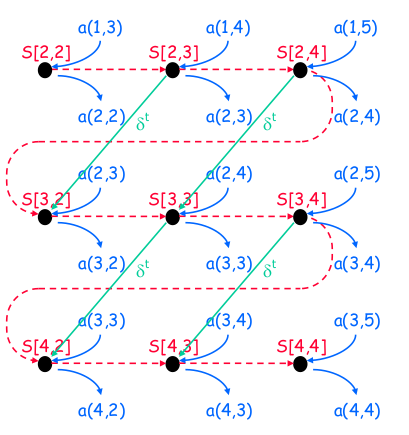
\includegraphics[width=0.3\textwidth]{p202.png}
	\caption{}
	\label{fig:p202}
\end{figure}


An instance of S precedes
another instance of S and
S produces data that S
consumes. S is both source and sink. The dependence is loop-
carried.
The dependence distance
is (1,-1). $S_1 \delta^{+}_{(1,-1)} S_2$


\subsection{LOOP TRANSFORMATIONS USING DIRECTION VECTORS}

\subsubsection{Loop Parallelization}

The iterations of a loop may be executed
in parallel with one another if and only if
no dependences are carried by the loop.

When that loop does not have a loop-carried dependence, it 
is safe to run a loop in parallel, which means
 outermost loop with a direction other than “=“

 \begin{figure}[H]
	\centering
	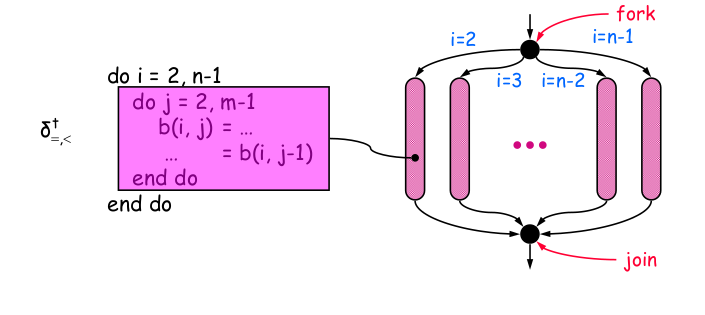
\includegraphics[width=0.3\textwidth]{p203.png}
	\caption{Iterations of loop j must be executed sequentially, but the
    iterations of loop i may be executed in parallel. Outer loop parallelism.}
	\label{fig:p203}
\end{figure}


\begin{figure}[H]
	\centering
	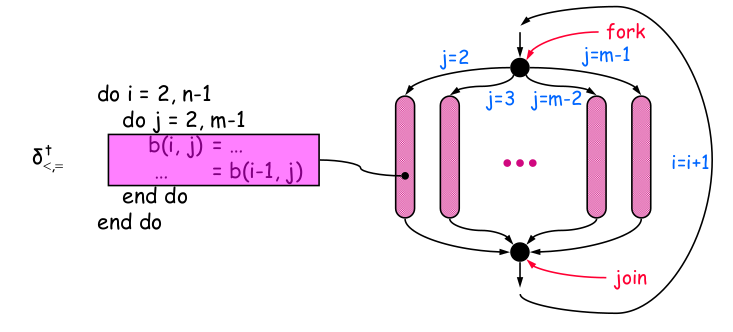
\includegraphics[width=0.3\textwidth]{p204.png}
	\caption{Iterations of loop i must be executed sequentially, but the
    iterations of loop j may be executed in parallel. Inner loop parallelism.}
	\label{fig:p204}
\end{figure}

\subsubsection{Loop Interchange}

When all dependences remain lexicographically positive,
it is legal to interchange or block/tile loops, which means
outermost direction other than “=“ must be “<” (positive)



\subsection{DATA DEPENDENCE DECISION ALGORITHM}


\subsubsection{Lamport's Test}

Lamport’s Test is used when there is a single index variable
in the subscript expressions, and when the coefficients of
the index variable in both expressions are the same.

\[ 
A(    \cdots    , b * i + c_1 ,    \cdots    ) =    \cdots   
   \cdots    = A(    \cdots    , b * i + c_2 ,    \cdots    )
\]


The dependence problem: does there exist i 1 and i 2 , such
that \(L_i \leq i_1 \leq i_2 \leq U_i \) and such that


\[ 
b * i_1 + c_1  =  b * i_2 + c_2
\]

or

\[ 
 i_2 - i _1 = \frac{c_1-c_2}{b_2} 
\]

There is integer solution if and only if \( \frac{c_1-c_2}{b_2}  \)is integer.
The dependence distance is \( d =  \frac{c_1-c_2}{b_2}  \) if \( L_i \leq |d| \leq U_i \)

\begin{itemize}

\item 	$d > 0$:  true dependence.
\item 	$d = 0$:  loop independent dependence.
\item 	$d < 0$:  anti dependence.
\end{itemize}


\begin{figure}[H]
	\centering
	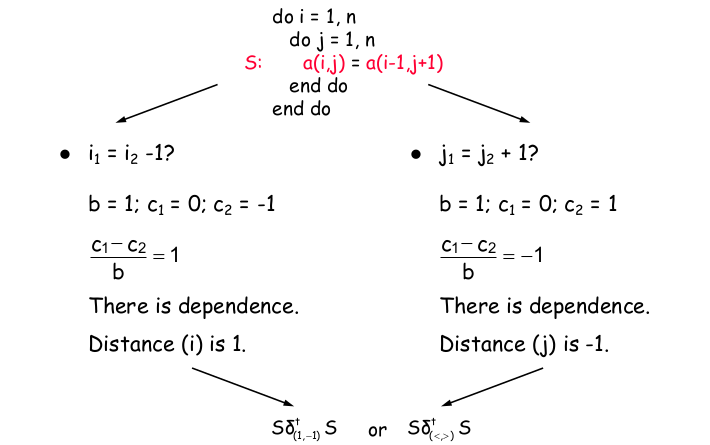
\includegraphics[width=0.3\textwidth]{p205.png}
	\caption{}
	\label{fig:p205}
\end{figure}

\begin{figure}[H]
	\centering
	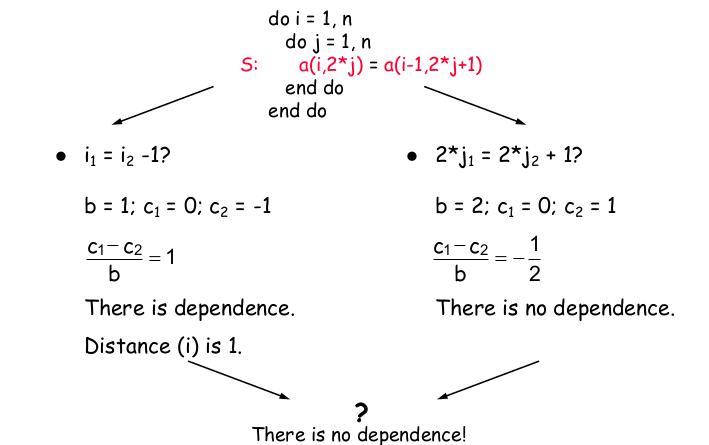
\includegraphics[width=0.3\textwidth]{p206.png}
	\caption{}
	\label{fig:p206}
\end{figure}

\subsubsection{GCD Test}
A greatest common divisor (GCD) test is 
a test used in computer science compiler theory to study of 
loop optimization and loop dependence analysis to test the dependency 
between loop statements. \cite{GCDtestW13:online}

It is difficult to analyze array references in compile time to 
determine data dependency (whether they point to same address or not). 
A simple and sufficient test for the absence of a dependence is 
the greatest common divisor (GCD) test. It is based on the observation 
that if a loop carried dependency exists between $X[a*i + b]$ and $X[c*i + d]$ 
(where X is the array; a, b, c and d are integers, and i is the loop variable),
 then GCD (c, a) must divide (d - b). The assumption is that the loop must
  be normalized : written so that the loop index/variable starts at 1 and 
  gets incremented by 1 in every iteration. For example, in the following
   loop, a=2, b=3, c=2, d=0 and GCD(a,c)=2 and (d-b) is -3. Since 2 
   does not divide -3, no dependence is possible.

\begin{lstlisting}[language=C,frame=single ,label = lst:expression1]
	for (i=1; i<=100; i++)
	{
	  X[2*i+3] = X[2*i] + 50;
	}
\end{lstlisting}